%%%%%%%%%%%%%%%%%%%%%%%%%%%%%%%%%%%%%%%%%%%%%%%%%%%%%%%%%%%%%%%%%%%%%%%%%
%%%%%%%%%%%%%%%%%%%%%%%%%      INTRODUÇÃO      %%%%%%%%%%%%%%%%%%%%%%%%%%
%%%%%%%%%%%%%%%%%%%%%%%%%%%%%%%%%%%%%%%%%%%%%%%%%%%%%%%%%%%%%%%%%%%%%%%%%

\section{\esp Introdução} \label{intro}

Instituída em 10 de dezembro de 2009, a Lei n.º 12.116/2009 \citeonline{lei}, conforme o Congresso Nacional Brasileiro, decreta o dia 27 de novembro como o Dia Nacional de Luta contra o Câncer de Mama. Além de uma data específica para a luta contra esse câncer, foi criada em 1990, uma campanha cujo objetivo é conscientizar a população sobre a importância da prevenção e do diagnóstico precoce, o chamado Outubro Rosa.

Causado pela multiplicação rápida e desordenada de células anormais, o câncer pode ocorrer em diversas estruturas do corpo, e quando envolve as células das glândulas mamárias, determina o câncer de mama \cite{incaoquee}. Esse tumor divide a primeira posição com o de pulmão no ranking dos cânceres mais incidentes do mundo, além de ser a doença mais comum entre as mulheres, na qual dados da Organização Mundial de Saúde (OMS) e do Instituto Nacional de Câncer (INCA) apontam que ocorrem por volta de 627 mil mortes por câncer de mama no mundo em 2018, sendo 17,7 mil no Brasil \cite{boletimepidemiologico}.

O diagnóstico prévio dessa doença tem alta significância na contenção do progresso da doença, devido à introdução antecipada do tratamento, que favorece o crescimento das chances de sobrevivência do paciente diagnosticado. Diante disso, existem alguns procedimentos basilares empregados para o diagnóstico dessa doença, tais quais: o exame de toque; exames clínicos; exames de imagens como a mamografia, ultrassonografia ou ressonância magnética; e a confirmação via biópsia.

% Problema Escolhido: já está incluso nesse parágrafo.
De acordo com \citeonline{mamografia}, a mamografia é o exame mais eficiente para a detecção do câncer de mama, sendo possível identificar o câncer em um estágio mais leve e curável. Perante o avanço computacional, a mamografia se destaca como uma técnica de diagnóstico que permite visualizar ossos e tecidos mais densos do corpo humano através de pequenas doses de radiação. Quando aplicada ao câncer de mama, a mamografia se torna uma ferramenta essencial para a detecção prévia da doença. Isso porque o câncer tende a apresentar características como massas com margens irregulares, nódulos, micro-calcificações e assimetrias \cite{detection}.

% Motivações
Com a evolução da computação em diversos âmbitos tecnológicos, tais como redes neurais, processamento de imagens e Inteligências Artificiais (IA), oportunidades foram criadas para investigar e implementar soluções avançadas na área da saúde, visando agregar a comunidade médica, além da sociedade no geral. Na oncologia, existem diversos métodos e práticas utilizadas para diagnosticar um quadro de câncer de um paciente, porém, em sua grande maioria, requer uma análise humana que é passiva de erros ou até mesmo incapaz de realizar predições, ou quantificar com precisão o diagnóstico do quadro clínico \cite{parametrization}.

Pautando-se na ideia de trazer ferramentas que auxiliam médicos no diagnóstico antecipado do câncer de mama, algoritmos de processamento de imagem e predição podem melhorar a tomada de decisões dos profissionais de saúde acerca do quadro geral dos pacientes. Dessa maneira, o tratamento pode ser iniciado previamente, podendo evitar a progressão do câncer para estágios mais avançados, que são mais difíceis de tratar, e aumentando as chances de cura, reduzindo a necessidade de tratamentos invasivos. À vista disso, os equipamentos desenvolvidos com esse propósito garantem uma qualidade de vida e longevidade maior para todos assolados pelo quadro de câncer.

% Objetivos
Diante do contexto levantado, o presente artigo apresenta uma metodologia para a identificação de células cancerosas, que utiliza o processamento e análise de mamografias por meio de Aprendizado por Transferência (do inglês \textit{Transfer Learning}). Outrossim, para investigar de maneira experimental o tema proposto neste artigo, foram utilizadas bases de dados, criteriosamente selecionadas e normalizadas em termos de tamanho e histograma, contendo amostras de mamografias para o treinamento de um algoritmo de IA desenvolvido. As amostras foram divididas em mamografias sem sinais de câncer e mamografias com câncer. Todos os códigos desenvolvidos e as bases de dados utilizadas estão disponíveis publicamente no \textit{GitHub}\footnote{\href{https://github.com/Vaftir/Breast-Cancer-Detection-AI-System}{\textit{https://github.com/Vaftir/Breast-Cancer-Detection-AI-System}}}.

Para criar um modelo de classificação binária (com câncer e sem câncer), foi utilizado o método de Aprendizado Profundo (do inglês \textit{Deep Learning}), que consiste em uma técnica avançada de Aprendizado de Máquina (do inglês \textit{Machine Learning}). Após o treinamento do modelo, sua acurácia foi avaliada por meio de testes, e assim que devidamente treinado, o algoritmo foi capaz de analisar as imagens dos exames mamográficos e realizar uma classificação precisa e automatizada do câncer de mama.

O restante deste artigo está estruturado da seguinte maneira: a Seção \ref{fundteorica} apresenta o referencial teórico, na Seção \ref{trabcorr} é fornecida uma visão geral dos trabalhos correlatos encontrados na literatura, a Seção \ref{metodologia} descreve a metodologia, dividida em materiais e métodos, e, por fim, a Seção \ref{results} apresenta os resultados preliminares. 


%%%%%%%%%%%%%%%%%%%%%%%%%%%%%%%%%%%%%%%%%%%%%%%%%%%%%%%%%%%%%%%%%%%%%%%%%
%%%%%%%%%%%%%%%%%%%      FUNDAMENTAÇÃO TEÓRICA       %%%%%%%%%%%%%%%%%%%%
%%%%%%%%%%%%%%%%%%%%%%%%%%%%%%%%%%%%%%%%%%%%%%%%%%%%%%%%%%%%%%%%%%%%%%%%%


\section{\esp Fundamentação teórica}  \label{fundteorica}

De modo a fornecer informações mais detalhadas sobre os tópicos vitais para a compreensão do presente artigo, esta seção retrata conceitos fundamentais sobre o câncer de mama, exames e tratamentos para a doença, bem como técnicas de processamento de mamografias. Além disso, será discutida a técnica de \textit{Deep Learning} com o uso de imagens para demonstrar sua relevância no contexto da detecção do câncer de mama.

%%%%%%%%%%%%%%%%%%%%%%      CÂNCER DE MAMA       %%%%%%%%%%%%%%%%%%%%%%%

\subsection{\esp Câncer de mama} \label{cancerdemama}
As células vivas que compõem o corpo humano se dividem para permitir o crescimento e a substituição de células danificadas ou mortas. A proliferação celular é regulada pelos genes do Ácido Desoxirribonucleico (DNA, do inglês Deoxyribonucleic Acid), transmitidos pelos pais e gerenciados para manter o equilíbrio no processo de divisão celular. O câncer, em geral, se forma quando esse controle genético é danificado ou perdido em uma, ou mais células que então continuam a se dividir normalmente, produzindo mais células anormais, causando danos a outros tecidos e funções corporais \cite{basicOncology}.

O câncer de mama, em específico, se dá pelo crescimento de células anormais na glândula mamária, e os sub-tipos diferentes desse câncer estão localizados sob o tecido adiposo (tecido que armazena gordura e mantém a maior reserva de energia do organismo) e no sistema ductal (ductos responsáveis por conduzir o leite até a papila). Conforme apontado por \citeonline{souza}, o câncer de mama apresenta células com uma taxa de duplicação de tamanho estimada em 4 meses. Embora o crescimento seja inicialmente lento, quando o tumor se torna palpável e não é tratado, o câncer pode se disseminar para os linfonodos, pulmões, ossos, fígado e cérebro, desenvolvendo metástase.

% A descoberta prévia do câncer de mama aumenta significativamente a probabilidade de um paciente se curar da doença, dependendo de qual método for utilizado para a detecção. Com isso, é necessário avaliar se o método escolhido é invasivo ou não. No passado, os equipamentos de medição de emissão infravermelha eram capazes de captar uma variação de temperatura apenas de 0,5 a 1 °C, utilizando uma tecnologia primitiva que exigia que um filme de cristal líquido fosse colocado nos seios dos pacientes para detectar a temperatura. Ainda assim, segundo \citeonline{noninvasive}, as câmeras de termografia infravermelhas digitais conseguem identificar mudanças de 0,08 °C, em adição de não demandar contato físico com o paciente.


%%%%%%%%%%%%%%%%%%%%%%     PROCESSAMENTO DE IMAGEM       %%%%%%%%%%%%%%%%%%%

\subsection{\esp Processamento de Imagem} \label{procesamentoimg}

Matematicamente, uma imagem pode ser descrita como uma função bidimensional, f(x, y), onde x e y representam coordenadas espaciais, e a amplitude de f em qualquer par de coordenadas é chamada de a intensidade ou nível de cinza da imagem naquele ponto \cite{techniques}. Quando x, y e os valores de intensidade de f são quantidades finitas e discretas, chamamos a imagem de digital. É essencial que uma imagem digital seja composta por um número finito de elementos (conhecidos como \textit{pixels}, \textit{pels} ou elementos de imagem), cada um com sua própria localização e valores específicos. 

A definição básica de processamento de imagem refere-se ao processo de tratamento de imagens digitais, incluindo a remoção de ruídos e outros tipos de irregularidades presentes \cite{histopathological}. Durante as últimas quatro a cinco décadas, várias técnicas foram desenvolvidas no campo de processamento de imagens, sendo a maioria elaborada para aprimorar imagens obtidas por espaçonaves não tripuladas, sondas espaciais e aeronaves militares de reconhecimento. Devido a fácil disponibilidade de computadores poderosos, dispositivos de memória de grande porte e software gráfico, os sistemas de processamentos de imagem estão se tornando cada vez mais populares. As principais vantagens dos métodos de processamento são versatilidade, repetibilidade e preservação da precisão dos dados originais, utilizando técnicas como: i) Pré-processamento, ii) Melhoria, iii) Segmentação, iv) Extração de recursos, e v) Classificação \cite{lungcancer}.

As imagens capturadas por satélites e câmeras convencionais ou digitais carecem de contraste e brilho devido a limitações nos subsistemas de imagem, ou condições de iluminação durante a captura. Além disso, segundo \citeonline{techniques}, essas imagens podem conter diferentes tipos de ruído. Nesse contexto, o aprimoramento de imagem procura acentuar certas características da imagem para análise posterior ou exibição. Os exemplos incluem contraste e retoque de borda, pseudo-coloração, filtragem de ruído, nitidez e ampliação. As técnicas de aperfeiçoamento, que englobam alargamento de contraste, conforme mostrado na Figura \ref{fig:contraste}, modificação do histograma e filtragem de ruído, consoante à Figura \ref{fig:ruido}, são úteis na extração de recursos, análise e exibição. Entretanto, o próprio processo de aprimoramento não aumenta o conteúdo de informações inerentes aos dados, enfatizando somente certas características de imagem especificadas. Algoritmos de aprimoramento são geralmente interativos e dependentes de aplicativos.

\begin{figure}[ht]
\centering
\begin{minipage}[b]{0.45\linewidth}
\centering
\caption{Alargamento de Contraste}
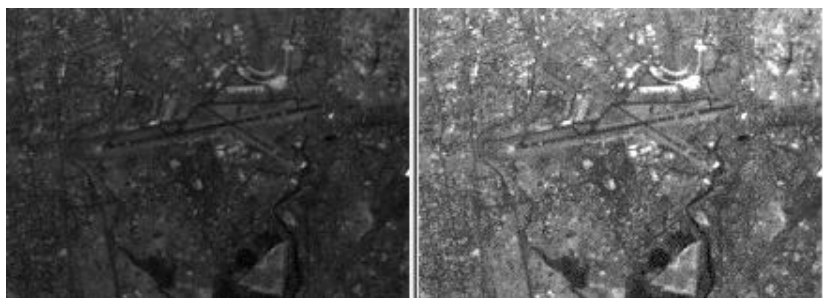
\includegraphics[width=\textwidth]{figuras/Alargamento de Contraste.png}
\label{fig:contraste}
\vspace{-0.2cm}
\textbf{\footnotesize Fonte: \cite{techniques}}
\end{minipage}
\hspace{0.5cm}
\begin{minipage}[b]{0.45\linewidth}
\centering
\caption{Retirada de Ruído}
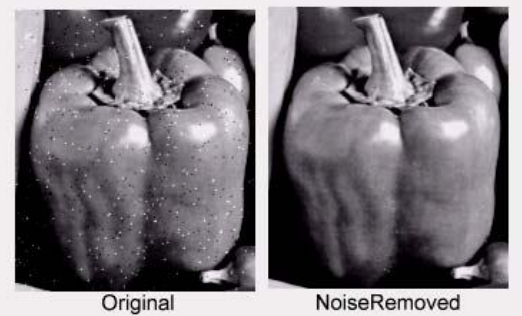
\includegraphics[width=\textwidth]{figuras/Retirada de Ruido.png}
\label{fig:ruido}
\vspace{-0.2cm}
\textbf{\footnotesize Fonte: \cite{techniques}}
\end{minipage}
\end{figure}



%%%%%%%%%%%%%%%%%%%%%%%%%%     DEEP LEARNING       %%%%%%%%%%%%%%%%%%%%%%

\subsection{\esp \textit{Deep Learning}} \label{deeplearning}

O \textit{Machine Learning} é um processo que utiliza uma gama de dados para criar uma IA instruído para aprender e operar funções de maneira autônoma \cite{machinelearning}. Dentre as abundantes formas de se aplicar esse processo, uma das mais comuns é o método \textit{Deep Learning}, que utiliza redes neurais convolucionais para criar aplicações mais completas. 

O termo \textit{Deep Learning} refere-se à estrutura utilizada para realização do método, que consiste em várias camadas de neurônios artificiais conectados, permitindo que o sistema aprenda representações cada vez mais complexas dos dados de entrada. Esses dados podem variar desde um simples conjunto de inteiros, para fazer uma predição de cálculo, até um sistema de navegação de um veículo autônomo \cite{deeplearning}.

Os neurônios artificiais são a principal composição da rede neural, sendo estruturas agrupadas em camadas, inspiradas nos neurônios biológicos presentes no cérebro humano. Cada neurônio artificial recebe diversas entradas, representadas por valores numéricos, multiplicadas por um determinado peso e somados. Esse resultado é então processado mediante uma função de ativação, que determina a saída do neurônio, e é transmitida para os outros neurônios da rede.



%%%%%%%%%%%%%%%%%%%%%%%%%%     REDES NEURAIS       %%%%%%%%%%%%%%%%%%%%%%


\subsection{\esp Redes Convolucionais} \label{redesneurais}

A Rede Neural Convolucional (CNN, do inglês \textit{Convolutional Neural Network}), de acordo com \citeonline{cnn}, é uma estrutura complexa composta por inúmeros neurônios e camadas de convolução compostas por um conjunto de filtros que, por sua vez, detectam características visuais específicas em uma imagem por meio de uma matriz. Sua arquitetura pode ser dividida em três camadas individuais: i) Camada de Entrada (do inglês \textit{Input Layer}), ii) Camadas Escondidas (do inglês \textit{Hidden Layers}), e iii) Camada de Saída (do inglês \textit{Output Layer}), com funções de entrada, processamento, e saída de dados respectivamente \cite{medical}.

Na camada de entrada, os dados brutos, como fotos e vídeos, são recebidos e transformados em dados matemáticos enviados para as camadas seguintes da CNN \cite{cnn}. Nas camadas escondidas, são usadas funções matemáticas não-lineares modeladas para retornar valores específicos, consoantes os dados de entrada. Esses valores são então enviados para a última parte da rede. Por fim, na camada de saída, é produzido o resultado com base nas predições das camadas anteriores.

% Figura \ref{fig:cnndrawio}
% \begin{figure}[ht]
%  	\centering	
%  	\caption[\hspace{0.1cm}Grade Computacional.]{Etapas metadológicas}
%  	\vspace{-0.2cm}
%  	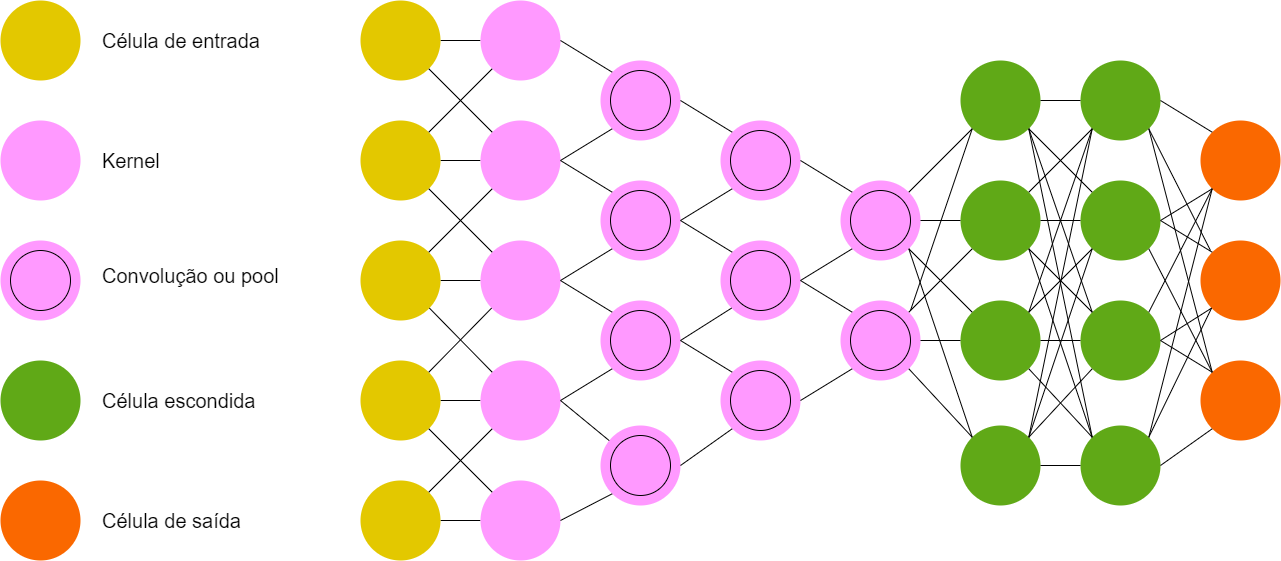
\includegraphics[width=1\textwidth]{figuras/cnn.drawio.png}
%     \captionsetup{justification=centering}
%   \vspace{-0.2cm}
%      \\\textbf{\footnotesize Fonte: Elaborado pelos autores}
% 	\label{fig:cnndrawio}
% \end{figure}

\subsection{\esp Redes Residuais} \label{redesresiduais}

As CNNs são amplamente reconhecidas por sua eficácia no tratamento de problemas de reconhecimento de imagem, oferecendo um elevado nível de precisão e escalabilidade. Essa popularidade resultou no desenvolvimento de diversas arquiteturas de CNN, cada uma abordando o problema de maneiras distintas. Dentro da ampla variedade de opções de arquiteturas de CNN, destacam-se exemplos como \textit{LeNet}, \textit{AlexNet}, \textit{ZFNet}, \textit{VGGNet}, \textit{ResNet}, \textit{GoogleLeNet}, entre outras. 

Uma Rede Neural Residual (ResNet, do inglês \textit{Residual Network}) representa uma arquitetura de CNN que permite melhorar a eficiência no treinamento e resolver problemas associados à degradação de desempenho. A \textit{ResNet} é capaz de navegar através de múltiplas camadas da rede, viabilizada pelo uso de atalhos. Adicionalmente, a arquitetura é composta por vários blocos residuais, que são retratados como uma construção especial que visa facilitar o treinamento de redes neurais, permitindo que a rede aprenda mudanças incrementais nas características. 

Dentro de cada bloco residual, várias camadas são empilhadas e o fluxo de dados é enriquecido pelos atalhos que permitem a passagem direta das informações às camadas subsequentes. Esses blocos variam em tipos e camadas, adaptando-se à profundidade e complexidade específicas da arquitetura. A Figura \ref{fig:cnn} ilustra as camadas de uma \textit{ResNet}, aplicado no problema de identificação de câncer de mama.

\begin{figure}[ht]
 	\centering	
 	\caption[\hspace{0.1cm}Grade Computacional.]{Arquitetura completa de uma CNN que classifica dígitos manuscritos}
 	\vspace{-0.2cm}
 	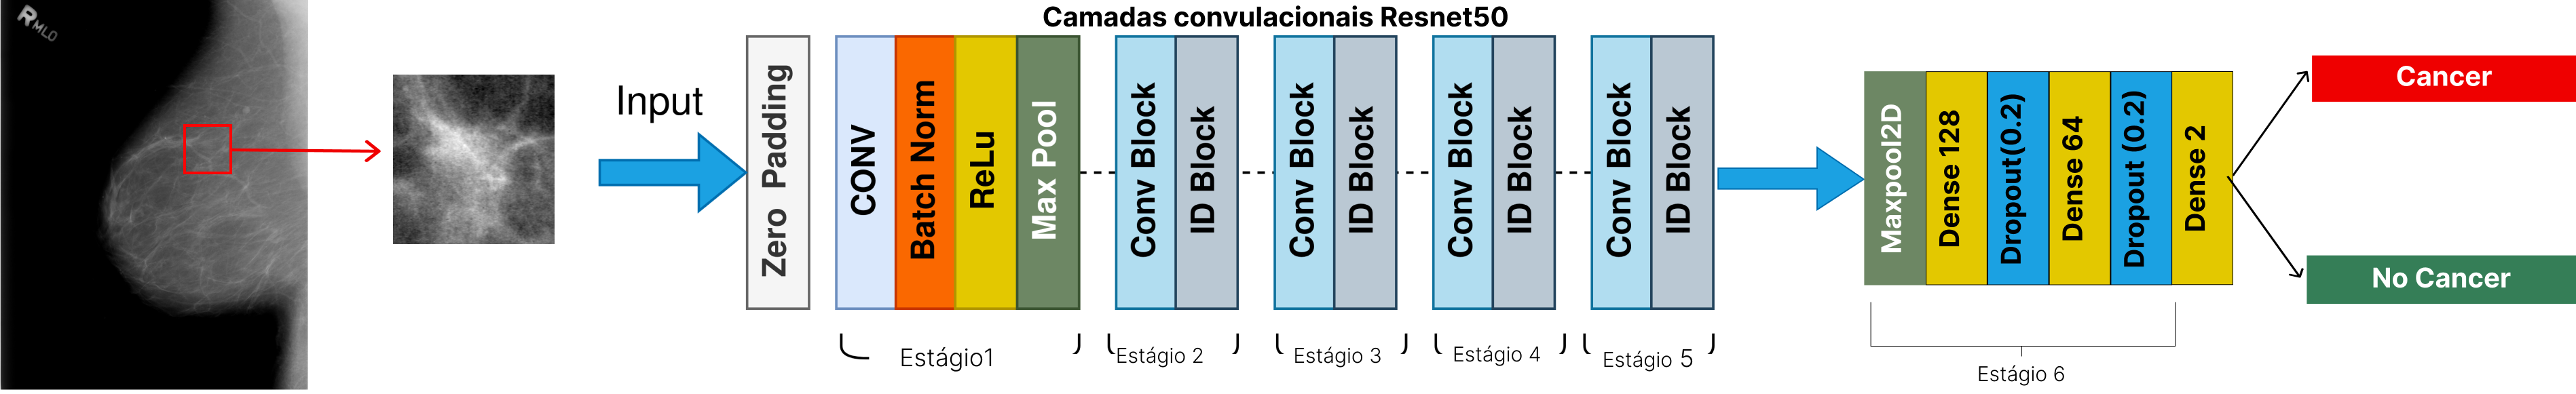
\includegraphics[width=1\textwidth]{figuras/cnn.png}
 	\captionsetup{justification=centering}
	\vspace{-0.2cm}
     \\\textbf{\footnotesize Fonte: Elaborado pelos autores}
	\label{fig:cnn}
\end{figure}

\subsection{\esp Camadas da CNN e Funções de Ativação} \label{camadasfund}

Uma arquitetura \textit{ResNet} é formada por diversos blocos residuais, em que cada bloco é composto por múltiplas camadas. A configuração dos blocos e camadas pode variar de acordo com a profundidade e complexidade da arquitetura em questão.

\subsubsection{\esp Camadas Convolucionais} \label{convs}

Cada bloco residual inicia com camadas convolucionais cuja função é aplicar um conjunto de filtros a uma imagem de entrada para extrair características importantes. A profundidade da saída de uma convolução corresponde ao número de filtros aplicados. Quanto mais profunda for a camada de convolução, mais detalhadas serão as características identificadas no Mapa de Ativação (do inglês \textit{Atactivation Map}), ou Mapa de Características. 

Os filtros, também conhecidos como \textit{Kernels}, consistem em pesos inicializados aleatoriamente, que são ajustados a cada nova entrada durante o processo de Retropropagação do Erro (do inglês \textit{Backpropagation}). A pequena região da entrada onde o filtro é aplicado é denominada Campo Receptivo (do inglês \textit{Receptive Field}). Na Figura \ref{fig:conv2} é possível observar um filtro que representa a curva ao seu lado. Essa combinação resulta em um valor alto, indicando compatibilidade entre as curvas. Quando não há compatibilidade na imagem, esse resultado se aproxima de zero.

\begin{figure}[ht]
 	\centering	
 	\caption[\hspace{0.1cm}Grade Computacional.]{Camada Convolucional}
 	\vspace{-0.4cm}
 	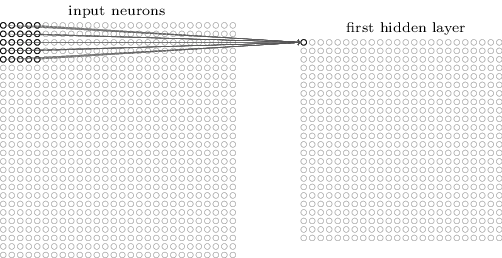
\includegraphics[width=1\textwidth]{figuras/conv.png}
 	\captionsetup{justification=centering}
	\vspace{-0.2cm}
     \\\textbf{\footnotesize Fonte: \cite{cnns}}
	\label{fig:conv2}
\end{figure}


\subsubsection{\esp Funções de Ativação} \label{funcAtiv}

Após as operações de convolução, são aplicadas funções de ativação. A função \textit{Softmax}, representada na Figura \ref{fig:softmax}, é comumente usada em redes neurais de classificação para tarefas de classificação. Ela tem a finalidade de forçar a saída da rede neural a representar a probabilidade de pertencimento dos dados a uma das classes predefinidas. Sem a função \textit{Softmax}, as saídas dos neurônios são simplesmente valores numéricos, onde o maior indica a classe vencedora. 

Em contrapartida, a função de ativação Unidade Linear Retificada (ReLU, do inglês \textit{Rectified Linear Unit}), representada na Figura \ref{fig:relu}, atribui o valor zero a todas as entradas menores ou iguais à zero. É amplamente utilizada devido à sua rapidez na geração de pesos e é especialmente adequada para problemas com apenas duas classes.

\begin{figure}[ht]
\centering
\begin{minipage}{0.45\textwidth}
  \centering
  \caption[\hspace{0.1cm}Grade Computacional.]{Função de Ativação \textit{softmax}}
  \vspace{-0.4cm}
  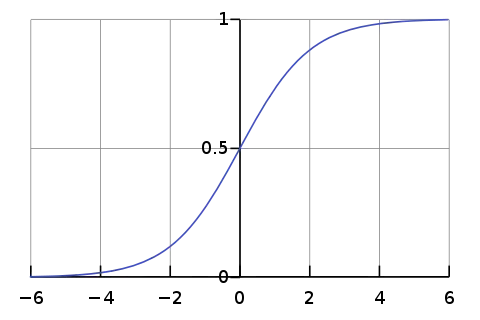
\includegraphics[width=\linewidth]{figuras/softmax.png}
  \captionsetup{justification=centering}
  \vspace{-0.2cm}
  \\\textbf{\footnotesize Fonte: \cite{softmax}}
  \label{fig:softmax}
\end{minipage}\hfill
\begin{minipage}{0.45\textwidth}
  \centering
  \caption[\hspace{0.1cm}Grade Computacional.]{Função de Ativação \textit{ReLU}}
  \vspace{-0.4cm}
  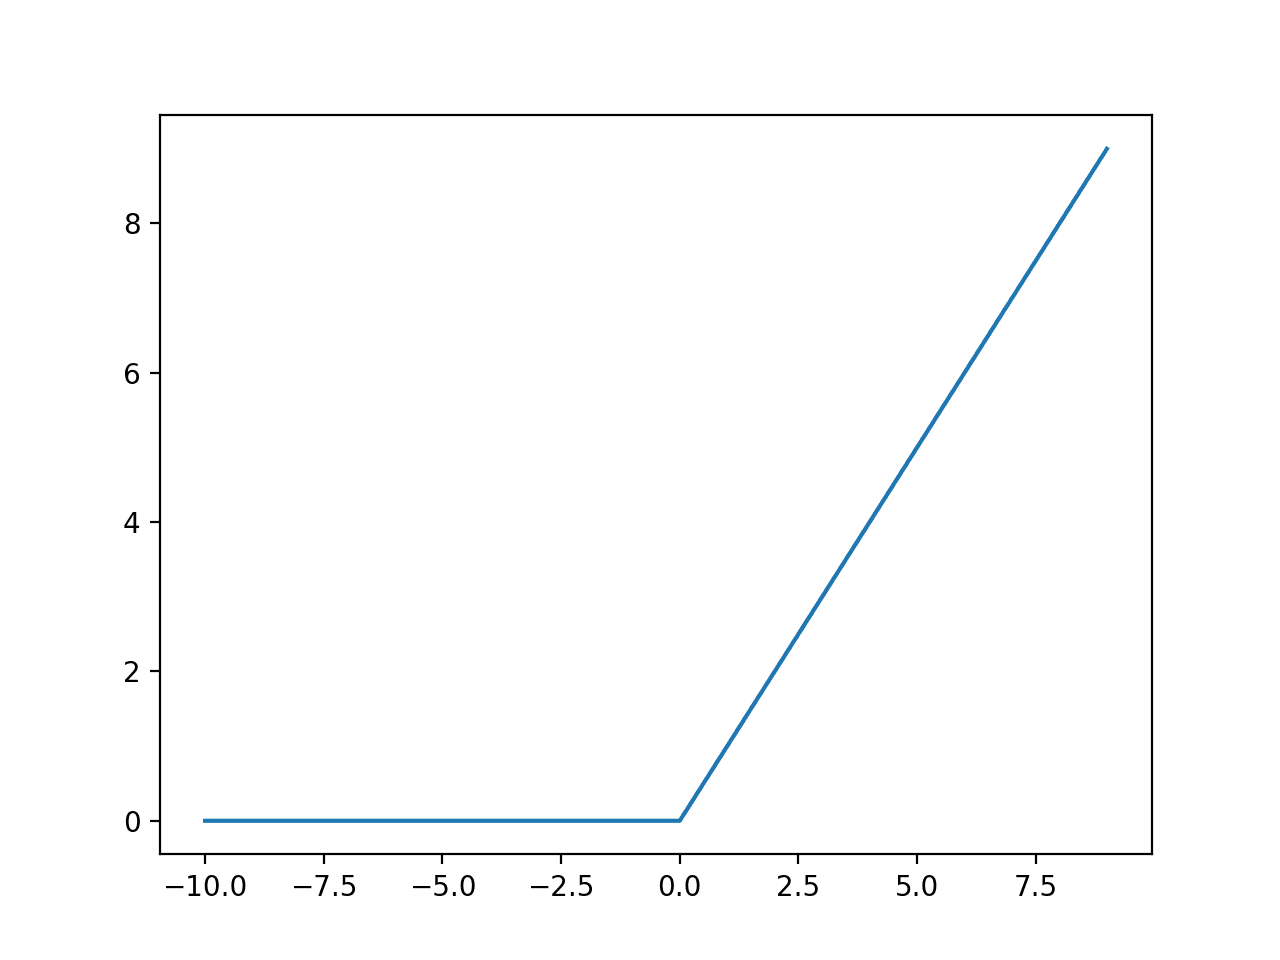
\includegraphics[width=\linewidth]{figuras/relu.png}
  \captionsetup{justification=centering}
  \vspace{-0.2cm}
  \\\textbf{\footnotesize Fonte: \cite{relu}}
  \label{fig:relu}
\end{minipage}
\end{figure}


\subsubsection{\esp Camadas de \textit{Pooling}} \label{convs}

A camada de \textit{Max Pooling} desempenha um papel importante na redução da dimensionalidade dos dados de entrada. Ela opera agrupando \textit{pixels} em regiões o que ajuda a reduzir a sensibilidade a pequenas variações nos dados, ao mesmo tempo em que extrai características mais relevantes. Essencialmente, essa camada diminui a resolução da imagem, permitindo uma ênfase maior em características específicas, enquanto compacta o conjunto de dados mantendo as informações mais relevantes em uma seleção das regiões de maior destaque.

\subsubsection{\esp Camadas \textit{Fully-Connected}} \label{fully}

Após os blocos residuais, a \textit{ResNet} possibilita a integração de camadas Totalmente Conectadas (do inglês, \textit{Fully-Connected}), também conhecidas como camadas \textit{Dense}. Essas camadas são responsáveis por tomar as características extraídas por camadas anteriores e transformá-las em uma saída final. No entanto, essas camadas não fazem parte dos próprios blocos residuais da \textit{ResNet}, uma vez que a arquitetura é focada em melhorar a eficácia das camadas convolucionais.

%%%%%%%%%%%%%%%%%%%%%%%%%%%%%%%%%%%%%%%%%%%%%%%%%%%%%%%%%%%%%%%%%%%%%%%%%
%%%%%%%%%%%%%%%%%%%%      TRABALHOS CORRELATOS       %%%%%%%%%%%%%%%%%%%%
%%%%%%%%%%%%%%%%%%%%%%%%%%%%%%%%%%%%%%%%%%%%%%%%%%%%%%%%%%%%%%%%%%%%%%%%%


\section{\esp Trabalhos correlatos} \label{trabcorr}

Nesta seção, são abordados trabalhos correlatos que utilizam IA para o diagnóstico de câncer, se diferenciando em termos de entrada de imagem (como radiografias ou imagens digitais), além de apresentar as bases de dados usadas, abordagens, algoritmos e análises dos resultados. 

Em \citeonline{marinePredators}, foi proposto um modelo de detecção de câncer de mama. O trabalho alcançou uma acurácia de 92\%, normalizando imagens termográficas e utilizando o \textit{Marine-Predators-Algorithm} que auxilia na otimização da seleção das características (definidas por algumas técnicas de reconhecimento de padrões) mais relevantes das imagens e parâmetros do modelo de observação. Para classificar e validar a implementação feita, foram utilizadas variantes (tipos de funções matemáticas que medem a similaridade entre dois pontos no espaço) do algoritmo de Máquina de Vetores de Suporte (SVM, do inglês \textit{Support Vector Machine}).

Por outro lado, \citeonline{comparing} ao utilizar outra abordagem de treinamento do algoritmo, chegaram em 61,8\% de precisão dos resultados. Foi utilizado o método de limiarização por refinamento adaptativo, técnica que segmenta uma imagem em duas ou mais (com base nos valores dos \textit{pixels}), de modo que regiões anormais são identificadas com mais precisão. Além disso, o artigo também comparou o resultado entre suas métricas com outros trabalhos, e com base nisso, concluiu-se que a inconsistência das comparações foi devido ao uso de imagens infravermelhas distintas, uma vez que foram utilizadas 102 imagens de uma base de dados pública.
%Diz q usa limiarização baseado na Section III .ASPECTS OF THE APPLIED APPROACH: "In our approach we have used the same methodology that composed the automatic ROI segmentation developed in [19] that was proven to produce good results regarding a comparison to a (...)"

Assim como o trabalho anterior, \citeonline{segmentacao} utilizaram da limiarização por refinamento adaptativo, todavia, com uma acurácia de 96\%. Foram introduzidos três parâmetros para avaliação, baseando-se na informação de que as pregas mamárias (área indicadora de limites inferiores da mama, pois possuem maior temperatura) podem variar de tamanho, dificultando a identificação das mamas. Os parâmetros determinam miliares mínimos de uma área medida em \textit{pixels} que a prega deve ter, além de definir a área mínima a ser medida em \textit{pixel} para duas componentes distintas. Com isso, foi possível determinar qual conjunto de parâmetros maximiza as métricas estatísticas apresentadas, indicando assim os resultados normalizados.

Como aplicado em \citeonline{MachineVision}, foram desenvolvidas técnicas de Visão de Máquina (do inglês \textit{Machine Vision}), algoritmo que processa imagens e reconhece características básicas, em contrapartida à técnicas de processamento de imagens, em que a saída é outra imagem, entretanto, devidamente tratada. Com o uso de linguagens de alto nível confiáveis e eficientes, inúmeros algoritmos foram otimizados resultando na criação de poderosas ferramentas acessíveis para pesquisadores e cientistas, aumentando a precisão dos resultados. A discussão da Visão de Máquina básica e algoritmos de processamento de imagem do artigo foram implementados em cinco grupos principais: 
\begin{enumerate}
  \renewcommand{\labelenumi}{\alph{enumi})}
    \item Técnicas de Segmentação ou Limiar em \textit{Grey-Level}: utilizando métodos como \textit{P-tile} (histogramas), \textit{Edge Pixel} e \textit{Interative};
    
    \item Técnicas de Detecção de Borda: localização da borda para aumentar o contraste, utilizando o algoritmo \textit{Canny Edge Detection};
    
    \item Morfologia Digital: filtra a imagem, além de fazer uma análise geométrica da estrutura dos elementos;
    
    \item Textura: observação da repetição de padrões a fim de substitui-los usando \textit{grey level};
    
    \item Algoritmos de Esqueletização e Encurtamento: definir propriedades globais dos objetos e reduzir a imagem em um modelo mais compacto para reconhecer padrões.
\end{enumerate}


Utilizando redes neurais para reconhecer imagens de câncer de pele e unindo técnicas de processamento de imagens digitais, \citeonline{botelho} possibilitaram a elaboração de um sistema que diferencia imagens de Melanomas. Para isso, quatro características são usadas para identificar uma lesão: assimetria, bordas irregulares, cor variada e diâmetro. Baseados nessas características, o modelo proposto implementa a rede neural \textit{Perceptron} de Camada Única, utilizando dois neurônios: um excitado por imagens de lesões Melanoma, e outro excitado por imagens de lesões não Melanoma. O \textit{Perceptron} identifica quando uma entrada é classificada erroneamente e ajusta os pesos por meio de uma regra de correção de erro, conhecida como Regra Delta. Com isso, a rede foi treinada somente quando todas as saídas corresponderam com a saída esperada, atingindo uma taxa de 69\% de acertos.

\citeonline{NakagamiImages} apresentam uma abordagem baseada em \textit{Deep Learning} para detecção e classificação de massas na mama combinando imagens de ultrassom \textit{B-mode} e Nakagami, para fornecer informações complementares sobre o padrão de dispersão de tecidos. O ultrassom B-mode consiste em uma técnica que utiliza ondas sonoras de alta frequência enviadas ao corpo, e refletidas pelos tecidos internos, criando uma imagem em escala cinza aonde as áreas mais brilhantes representam tecidos mais densos. Já as imagens Nakagami são geradas a partir da análise das amplitudes de sinal retornadas pelo tecido examinado, fornecendo informações sobre a presença de diferentes tipos de estruturas. Utilizando uma arquitetura de rede neural convolucional para extrair características das imagens combinadas, as massas foram classificadas como malignas ou benignas. Por fim, a abordagem proposta foi provada altamente eficaz na localização de massas, com uma precisão de 91,8\%, um desempenho significativamente melhor do que as abordagens existentes que usam apenas imagens B-mode ou Nakagami.

Em \citeonline{systematic}, os autores analisaram os diferentes tipos de Redes Neurais Artificiais (ANN, do inglês \textit{Artificial Neural Network}) e modelos de \textit{Deep Learning} já utilizados na literatura para processar imagens termográficas de câncer de mama. Mesmo que a termografia, seja atualmente o melhor método para a descoberta precoce, a qualidade das imagens é um desafio tangível. O processo de melhoramento da imagem tenta mostrar detalhes escondidos e destacar características para que a profundidade e tamanho do tumor sejam distinguidos de um tecido saudável. Para melhorar a qualidade da imagem, o trabalho utiliza um dispositivo de resfriamento de mama. Além disso, foram destacadas as contribuições e desvantagens de trabalhos relacionados que empregam termografia e IA, obtidos mediantes comparações feitas no decorrer do artigo e são desenvolvidos questionamentos a cerca dos desafios enfrentados, como a falta de padronização na aquisição de imagens térmicas e a necessidade de mais dados de treinamento para as redes neurais. 

Para desenvolver uma técnica precisa e eficiente para a identificação antecipada do câncer de mama, \citeonline{ChaoticSalp} usaram a segmentação de imagens térmicas em conjunto com o algoritmo \textit{Chaotic Salp Swarm}. O algoritmo proposto consiste em uma técnica de otimização bioinspirada, usada para ajustar os parâmetros de segmentação das termografias e encontrar as regiões suspeitas de câncer de mama. Assim como o anterior, foi utilizada uma base de dados pública de imagens térmicas para avaliar a eficácia do método proposto. Os resultados obtidos foram avaliados baseados em métricas como: sensibilidade, especificidade e coeficiente de Dice. Não foi especificado o índice de precisão do trabalho, entretanto, foi considerado que o método proposto teve um desempenho satisfatório em termos de precisão na segmentação de regiões suspeitas de câncer de mama nas imagens térmicas.

\citeonline{borchartt} teve como foco a análise das potenciais contribuições que o uso de imagens infravermelhas tem para diagnósticos de doenças na mama. Para o estudo, foram utilizadas 102 imagens Infravermelhas (IR, do inglês \textit{Infrared Radiation}) de mama única da base de dados público da Pro Engenharia (PROENG) (sendo 47\% com alguma anormalidade) e resultados foram obtidos através do uso de algoritmos para detecção de condições malignas, como SVM, para extrair as características como primeiro momento, terceiro momento, não uniformidade da massa cinzenta e porcentagem de execução. Os autores expuseram a dificuldade em realizar o processo de segmentação da região da mama, extração da região de interesse, devido à natureza amorfa e a falta de limites claros. Além disso, foi apontado que ao usar uma base de dados público para comparar as imagens e extrair características, os melhores resultados foram obtidos com o classificador \textit{Sequential Minimum Optimization} (SMO), em adição a expor a inconsistência da comparação entre trabalhos que utilizam imagens IR. 

Buscando explorar métodos não invasivos para a localização precoce do câncer de mama, \citeonline{leles} propuseram o uso de imagens térmicas que permitem detectar mudanças na temperatura, causadas pelo aumento do fluxo sanguíneo na área afetada pelo tumor. Após o pré-processamento, foi feito o refinamento manual da região de interesse para que alguns atributos extraídos não colaborassem com dados de fora da mama. Avaliando 70 pacientes, o trabalho identificou a temperatura máxima, mínima e média das mamas para utilizar no cálculo da sensibilidade (capacidade do teste em identificar corretamente o diagnóstico) e especificidade (capacidade do teste em excluir corretamente os que não tem a doença), com os valores de 92,3\% e 86,2\%, respectivamente.

A fim de abordar a detecção de metástase em linfonodos axilares em pacientes com câncer de mama, \citeonline{ashokkumar} utilizaram o método de \textit{Data Augmentation} que faz modificações geométricas das imagens (como rotação, inversão, deslocamento e dimensionamento). Isso fornece uma garantia de que o modelo se concentra em áreas de câncer de mama, em vez de fontes de ruído aleatórias. Conforme o texto, foi demonstrado que o método ajuda na memorização de qualidades específicas das imagens treinadas, e evita que as redes se tornem superajustadas, ou seja, um modelo de Aprendizado Profundo que se adaptou demasiadamente nos dados de treinamento a ponto de não conseguir capturar padrões mais amplos. Além disso, usando ANN, o trabalho alcançou 98\% de acurácia superando modelos de radiografia.


%%%%%%%%%%%%%%%%%%%%%%%%%%%%%%%%%%%%%%%%%%%%%%%%%%%%%%%%%%%%%%%%%%%%%%%%%
%%%%%%%%%%%%%%%%%%%%%%%%      METODOLOGIA       %%%%%%%%%%%%%%%%%%%%%%%%%
%%%%%%%%%%%%%%%%%%%%%%%%%%%%%%%%%%%%%%%%%%%%%%%%%%%%%%%%%%%%%%%%%%%%%%%%%


\section{\esp Metodologia} \label{metodologia}
A fim de aprofundar os fundamentos do tema abordado, esta seção apresenta os recursos e ferramentas utilizados para a implementação do algoritmo, bem como informações técnicas relacionadas a linguagens de programação, bibliotecas e base de dados.


%%%%%%%%%%%%%%%%%%%%%%%     MATERIAIS       %%%%%%%%%%%%%%%%%%%%%%

\subsection{\esp Materiais} \label{materiais}


%%%%%%%%%%%%%%%%%%%%%%%     BASE DE DADOS       %%%%%%%%%%%%%%%%%%%%%%
\subsubsection{\esp Base de Dados} \label{database}

%%%%%
As amostras de imagens mamográficas foram adquiridas a partir do desenvolvimento mencionado em \citeonline{newdatabase}, cujo objetivo é enfrentar o desafio comum associado a bancos de dados de imagens de mamografia, sejam eles de origem privada ou pública, caracterizados por seu tamanho limitado e restrições de acessibilidade, frequentemente dispondo de informações insuficientes.

O Subconjunto de imagens de mama com curadoria DDSM\footnote{\href{https://www.kaggle.com/datasets/awsaf49/cbis-ddsm-breast-cancer-image-dataset}{\textit{https://www.kaggle.com/datasets/awsaf49/cbis-ddsm-breast-cancer-image-dataset}. Acesso em 13 de setembro de 2023.}} (do inglês, \textit{Curated Breast Imaging Subset DDSM}), desenvolvido em 2016, conta com imagens de x pacientes com câncer e x pacientes sem câncer, totalizando x pacientes. Cada paciente possui, em média, y imagens capturadas em diferentes posições, incluindo frontal, lateral direita, lateral esquerda e outros ângulos. Para ilustrar, a Figura \ref{fig:pcc} demonstra um exemplo de uma imagem utilizada para a predição de um paciente com câncer, enquanto a Figura \ref{fig:psc} exibe uma imagem de um paciente sem câncer. 

% \footnote{\href{https://www.kaggle.com/datasets/awsaf49/cbis-ddsm-breast-cancer-image-dataset}{\textit{https://www.kaggle.com/datasets/awsaf49/cbis-ddsm-breast-cancer-image-dataset}. Acesso em 13 de setembro de 2023.}}

\begin{figure}[ht]
\centering
    \begin{minipage}[b]{0.45\textwidth}
        \centering
        \caption{Paciente com câncer}
        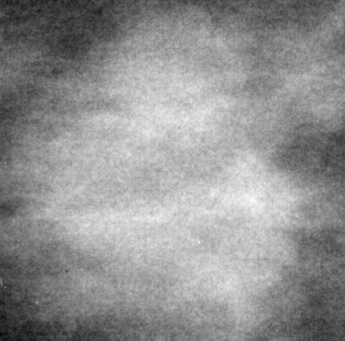
\includegraphics[width=0.5\textwidth]{figuras/with_cancer.jpg}
        \label{fig:pcc}
        
        \textbf{\footnotesize Fonte: \href{https://www.kaggle.com/datasets/awsaf49/cbis-ddsm-breast-cancer-image-dataset}{\cite{newdatabase}}}
    \end{minipage}
    \hfill
    \begin{minipage}[b]{0.45\textwidth}
        \centering
        \caption{Paciente sem câncer}
        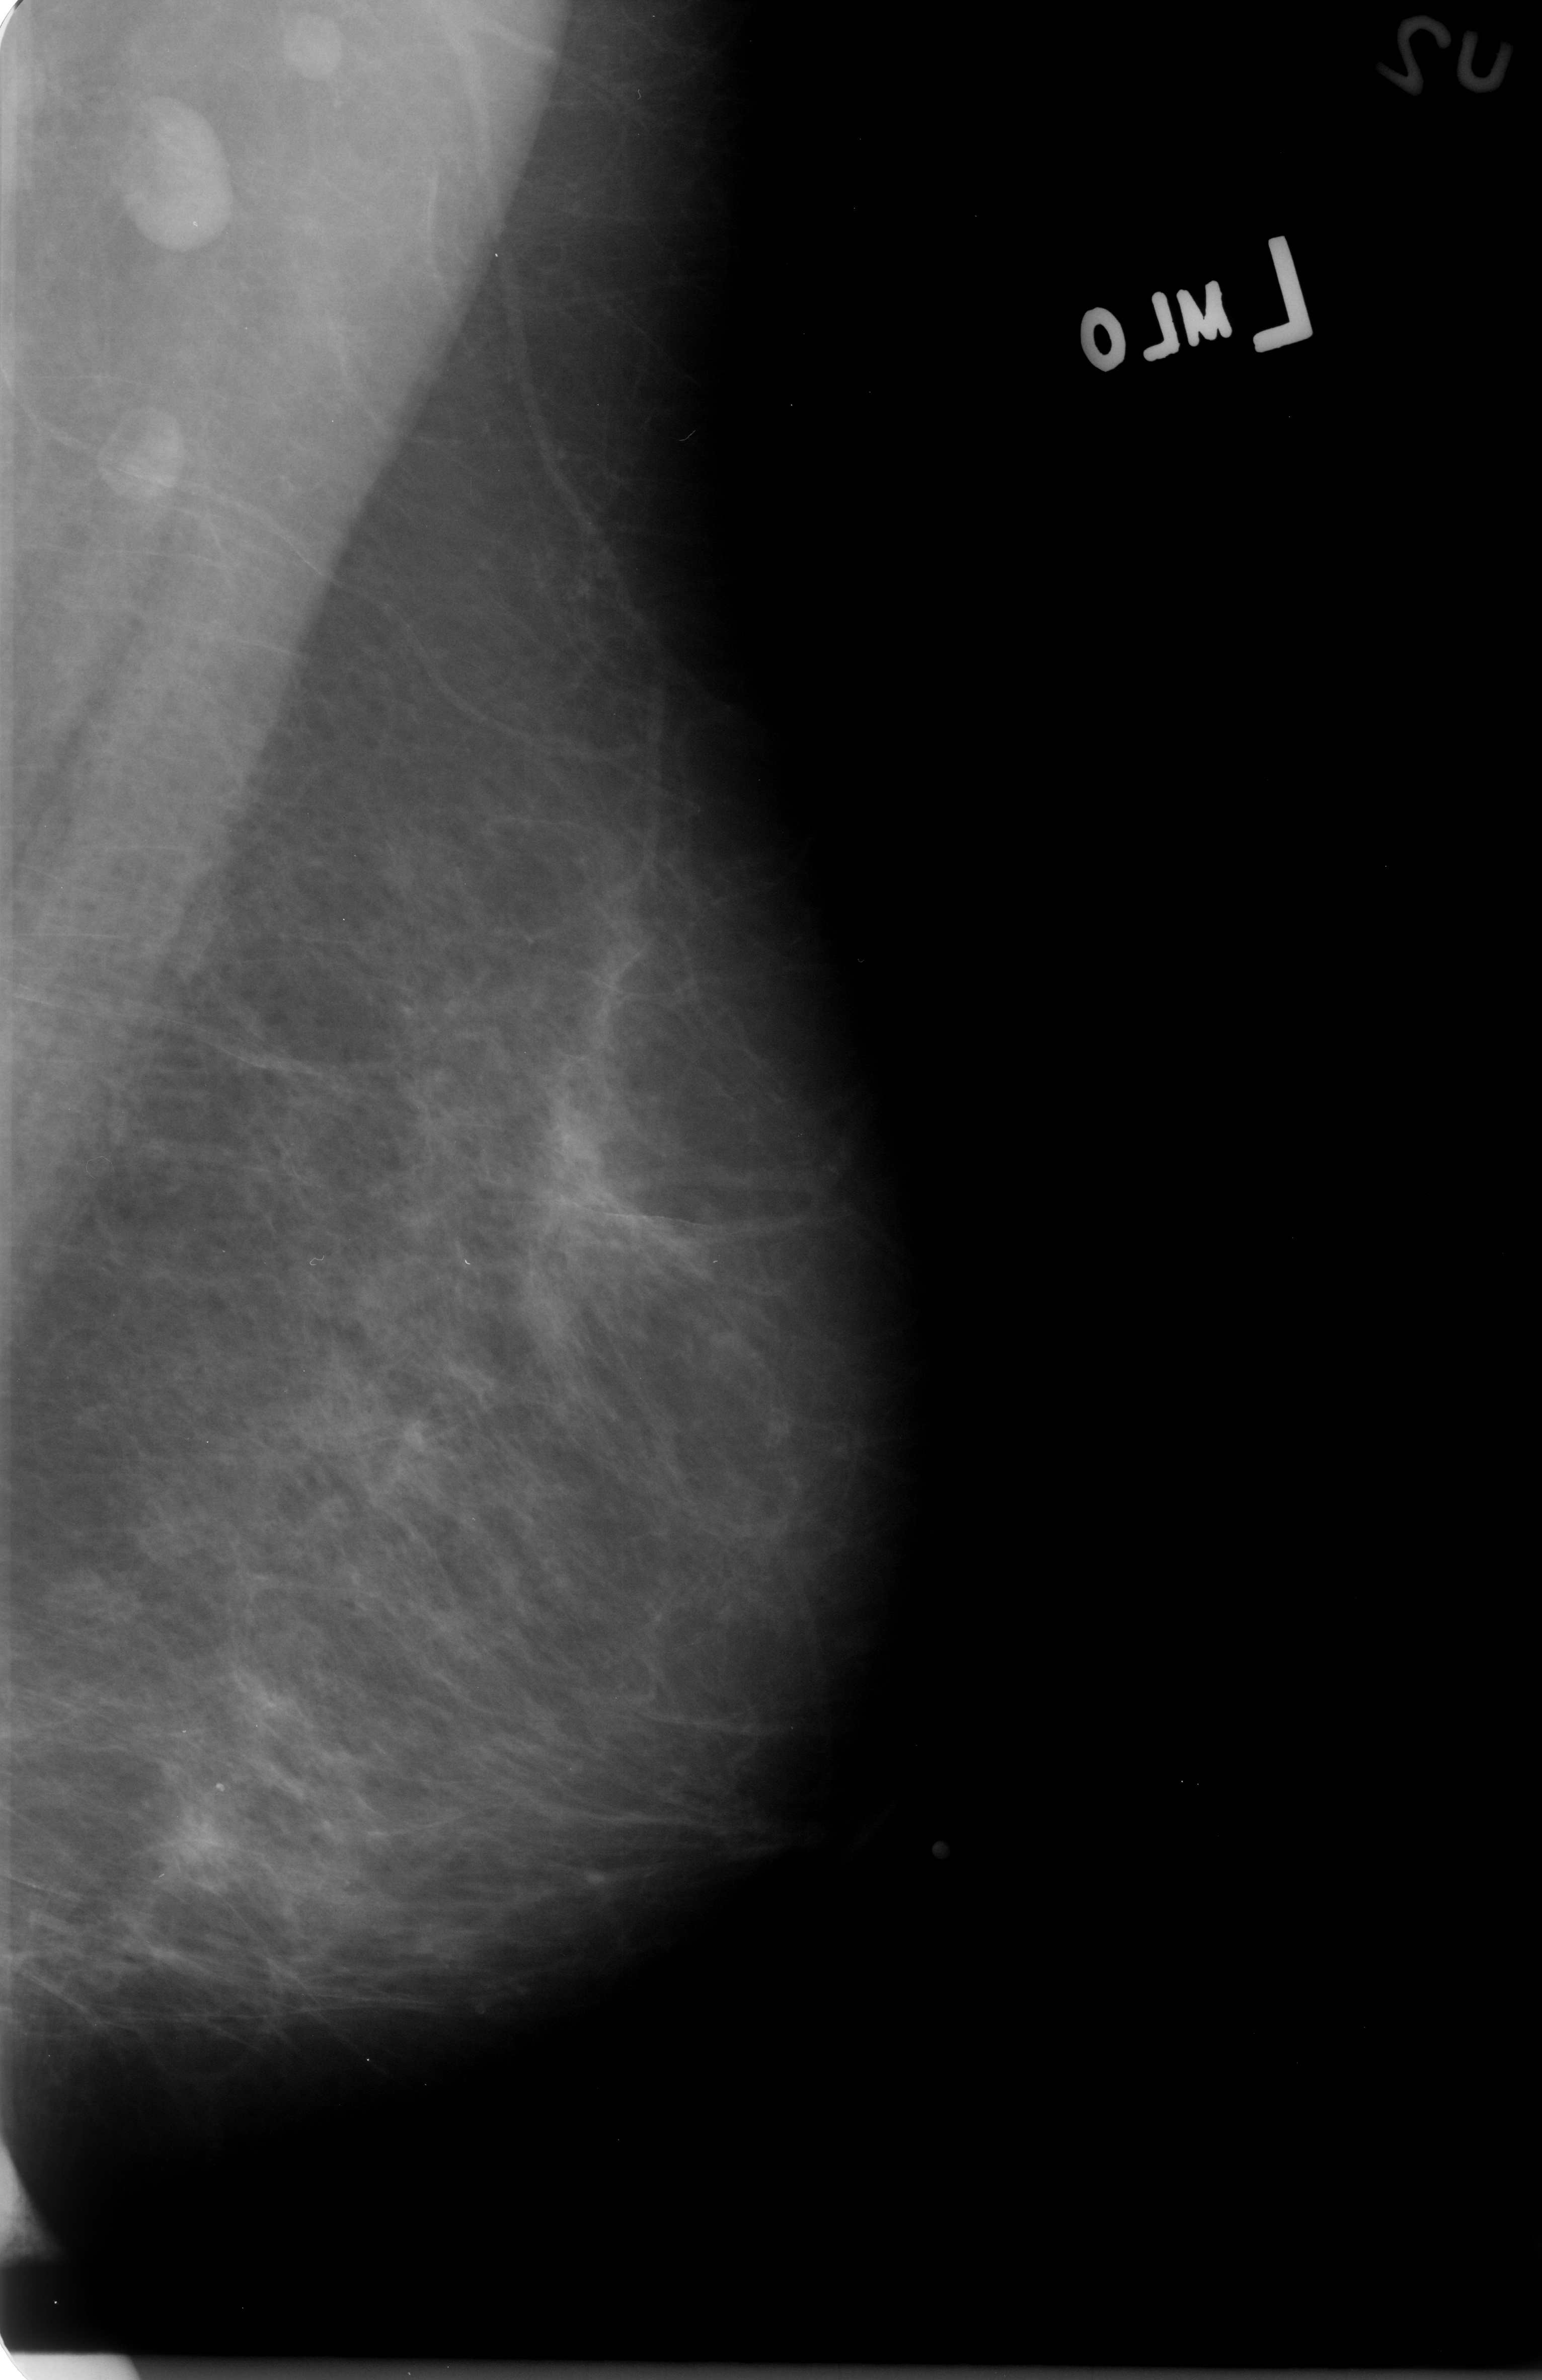
\includegraphics[width=0.5\textwidth]{figuras/without_cancer.jpg}
        \label{fig:psc}
        
        \textbf{\footnotesize Fonte: \href{https://www.kaggle.com/datasets/awsaf49/cbis-ddsm-breast-cancer-image-dataset}{\cite{newdatabase}}}
    \end{minipage}
\end{figure}



%%%%%%%%%%%%%%%%%%%%%%%     TECNOLOGIAS       %%%%%%%%%%%%%%%%%%%%%%

\subsubsection{\esp Tecnologias} \label{techs}
Para desenvolver o algoritmo de classificação das imagens entre pacientes com câncer e pacientes sem câncer, foram empregadas diversas tecnologias e bibliotecas, em conjunto com uma linguagem de programação, visando facilitar o processo. Para reproduzir a implementação, foi necessário configurar o sistema operacional do computador com o \textit{Python}, uma linguagem de programação de alto nível, interpretada e com tipagem dinâmica, além de incluir orientação a objetos, diversas bibliotecas e suporte a módulos e pacotes. A implementação foi realizada usando o \textit{Python} 3.10. Algumas das principais bibliotecas utilizadas são:

% Adicionalmente, para gerenciar as dependências do projeto, foi utilizado um gerenciador de pacotes para o \textit{Python} (por exemplo, utilizando o comando "\textit{pip install <pacote>}", onde <pacote> representa o nome do pacote a ser instalado). 

\begin{enumerate}[label=\alph*)]
    \item \textit{TensorFlow}: desenvolve modelos de \textit{Machine Learning}.
    
    \item \textit{Keras}: usada em conjunto com o \textit{TensorFlow}, permitindo construção e treinamento de redes neurais.
    
    % \item \textit{PIL}: oferece recursos para o processamento de imagens, como abrir, manipular e salvar em diferentes formatos.
        
    \item \textit{matplotlib}: para visualização de dados, permitindo criar gráficos, \textit{plots}, histogramas, entre outros.
    
    \item \textit{numpy}: aplicada para computação e análise numérica, fornecendo uma estrutura de dados como vetores multidimensionais para armazenar grandes conjuntos de dados numéricos.

    % \item \textit{os}: interage com o sistema operacional, permitindo manipulação de diretórios, entre outros.

    \item \textit{cv2}: fornece funções para carregar, manipular e processar imagens.

    % \item \textit{time}: medição de tempo e manipulação de datas.

    % \item \textit{glob}: realiza operações de pesquisa de arquivos e diretórios.

    % \item \textit{random}: gera números aleatórios e funções de aleatoriedades.

     \item \textit{ImageDataGenerator}: Originada do TensorFlow, permite transformar as imagens em dados vetoriais, facilitando os cálculos necessários durante o treinamento do modelo.
\end{enumerate}

\subsubsection{\esp Arquitetura de CNN} \label{arqCNN}

Apresentada na Subseção \ref{redesresiduais}, a arquitetura \textit{ResNet} destaca-se por sua ênfase no reconhecimento de imagens, além de ter conquistado o primeiro lugar no Desafio de Reconhecimento Visual em Larga Escala ImageNet (ILSVRC, do inglês \textit{ImageNet Large Scale Visual Recognition Challenge}) em 2015 \cite{resnet50analisys}. Neste desafio, obteve uma taxa de erro top 5 de 3,6\% ao empregar uma CNN composta por 152 camadas, denominada \textit{ResNet152}.

No entanto, apesar do prestígio da \textit{ResNet152} como o modelo mais profundo, capaz de capturar recursos abstratos e complexos, essa profundidade também traz consigo um peso significativo em termos computacionais. Isso a torna mais custosa tanto no treinamento quanto na implementação em dispositivos com recursos limitados. A família de variantes \textit{ResNet} inclui modelos que aderem ao mesmo conceito, mas diferentes quantidades de camadas, como \textit{ResNet18}, \textit{ResNet34}, \textit{ResNet50} e \textit{ResNet101}. 

Dentre essas, a \textit{ResNet50} se destaca por ter um equilíbrio na profundidade das camadas. Conforme indicado por \citeonline{resnet50analisys}, as \textit{ResNet} com 50, 101 e 152 camadas demonstram maior precisão em comparação às versões com 18 e 34 camadas. Ao reduzir as opções para 50, 101 e 152 camadas, foi possível definir a \textit{ResNet50} como a escolhida, uma vez que as arquiteturas com 101 e 152 camadas demandam recursos computacional mais substanciais do que aquela com 50 camadas.



%%%%%%%%%%%%%%%%%%%%%%%     MÉTODOS       %%%%%%%%%%%%%%%%%%%%%%


\subsection{\esp Métodos} \label{metodos}

Nesta subseção, são apresentadas as metodologias para o treinamento de um modelo de rede neural convolucional fazendo uso de bibliotecas do \textit{Python}. Disponíveis na Figura \ref{fig:diagrama}, o método proposto consiste em cinco etapas: base de imagens, pré-processamento, aplicação do método de \textit{Transfer Learning}, declaração do modelo e predições.

\begin{figure}[ht]
 	\centering	
 	\caption[\hspace{0.1cm}Grade Computacional.]{Etapas metodológicas}
 	\vspace{-0.2cm}
 	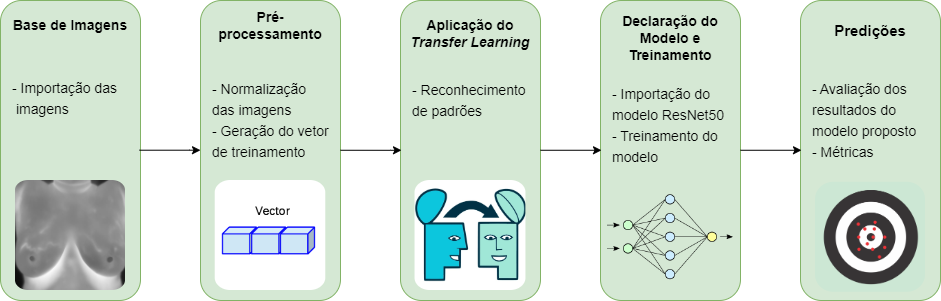
\includegraphics[width=1\textwidth]{figuras/tcc_diagrama.drawio.png}
    \captionsetup{justification=centering}
  \vspace{-0.2cm}
     \\\textbf{\footnotesize Fonte: Elaborado pelos autores}
	\label{fig:diagrama}
\end{figure}



%%%%%%%%%%%%%%%%%%%%%%%     PRÉ-PROCESSAMENTO       %%%%%%%%%%%%%%%%%%%%%%

\subsubsection{\esp Pré-Processamento} \label{preprocess}
Inicialmente, foram carregadas 206 imagens como dados de treinamento (sendo 103 para pacientes sem câncer e 103 para paciente com câncer), 60 imagens como dados de validação (sendo 30 para pacientes sem câncer e 30 para pacientes com câncer), e 12 imagens para dados de teste (sendo 6 para pacientes sem câncer e 6 para pacientes com câncer). Totalizando 278 imagens, foi feita a divisão entre imagens para treinamento em 74,1\%, validação em 21,6\% e teste em 4,3\%.

Em seguida, o pré-processamento das imagens foi realizado. Foram utilizados métodos que realizam a normalização dos valores dos \textit{pixels} das imagens, transformando os valores originais dos \textit{pixels} em uma escala específica. Geralmente, essa escala é utilizada com o valor de 1/255, uma vez que as imagens utilizadas na implementação consistem em coeficientes Vermelho, Verde, Azul (RGB, do inglês \textit{Red, Green, Blue}), ou seja, cada \textit{pixel} tem um valor entre 0 e 255. Entretanto, esses valores são grandes demais para o modelo proposto processar, conforme a taxa de aprendizado comum. Por conta disso, os valores foram realinhados para se distinguir entre 0 e 1.

Além disso, foi utilizado um método originado da biblioteca \textit{Keras} para pré-processar os dados carregados para o treinamento. Nesse método, foi realizado o redimensionamento das imagens para 224x224, uma vez que a \textit{ResNet} requer esses valores \cite{kerasresnet50}, além da criação de um gerador que fornece lotes de imagens conforme o necessário durante o treinamento do modelo.

%%%%%%%%%%%%%%%%%%%%%%%     TRANSFER LEARNING       %%%%%%%%%%%%%%%%%%%%%%

\subsubsection{\esp \textit{Transfer Learning}} \label{transfer}

A fim de empregar um modelo pré-treinado em uma determinada tarefa como ponto de partida para resolver um problema relacionado, o \textit{Transfer Learning} foi aplicado. Isso permite aproveitar o conhecimento adquirido por um modelo já pré-treinado, a fim de reconhecer padrões e características úteis nos dados. 

O método de aplicação consiste em obter camadas de um modelo já treinado, congelar essas camadas já treinadas (para evitar destruir quaisquer informações que elas possuem durante o treinamento), adicionar novas camadas treinadas em cima das camadas congeladas (retornando características anteriores em predições para um novo \textit{dataset}) e, por fim, treinar as novas camadas \cite{kerastransfer}.

Na implementação do modelo de classificação de câncer, foi utilizada a arquitetura \textit{ResNet50} para realizar o processo de \textit{Transfer Leaning}, modelo de rede neural que utiliza blocos residuais, permitindo que a informação seja passada diretamente para camadas posteriores. Com essa informação, foi carregado o pré-processamento da \textit{ResNet} para que as imagens possam ser entendíveis para a rede utilizada. Em seguida, foi utilizado um método para pré-processar novamente os dados que foram carregados para o treinamento e para a validação.


%%%%%%%%%%%%%%%%%%%%%%%     FUNÇÕES DE ATIVAÇÃO       %%%%%%%%%%%%%%%%%%%%%%

\subsubsection{\esp Importação do Modelo de Rede Neural} \label{camadas}

Com as imagens de treinamento e validação pré-processadas, procedeu-se com a incorporação da rede neural \textit{ResNet50} que aplica a técnica de \textit{Transfer Learning}. O modelo pré-treinado foi carregado, ajustando os parâmetros para excluir a camada superior do modelo, usando somente camadas convolucionais (camadas que fazem a extração dos atributos).

Como citado na Subseção \ref{fully}, a \textit{ResNet} por mais que completa, disponibiliza os dados extraídos mas não implementa as camadas \textit{Fully Connected}. Como o modelo base contém somente camadas Convolucionais, foi feito um procedimento onde todas as camadas do modelo \textit{ResNet50} não fossem treinadas durante o processo de treinamento subsequente. Ao definir isso, as camadas do modelo base permaneceram com os pesos pré-treinados e não foram atualizadas durante o treinamento adicional. 

Com base no modelo pré-treinado da \textit{ResNet50}, foi criado um modelo sequencial, com uma lista de camadas. Dentre elas, foi adicionada uma camada de \textit{Max-Pooling} global médio 2D que reduz a dimensionalidade dos recursos extraídos pelas camadas anteriores. Além disso, foram adicionadas quatro camadas \textit{Fully-Connected} realizando transformações lineares nos dados de entrada. Dentre elas, três são \textit{Hidden Layers} e somente uma é \textit{Output Layer}.

As \textit{Hidden Layers} foram definidas com 1024, 128 e 36 neurônios, em conjunto com a função de ativação ReLU. Uma quantidade maior de neurônios em uma camada intermediária proporcionam à rede mais capacidade de aprender representações complexas e abstratas dos dados. Já a \textit{Output Layer} foi definida com somente 2 neurônios, que corresponde o número de classes em um problema de classificação (ou seja, uma classificação binária), em conjunto com a função de ativação \textit{Softmax}.

%%%%%%%%%%%%%%%%%%%%%%%     TREINAMENTO       %%%%%%%%%%%%%%%%%%%%%%

\subsubsection{\esp Treinamento do Modelo} \label{treinamento}

A fim de treinar o modelo para identificar padrões e classificar as imagens, o modelo foi compilado para treinamento utilizando uma função de otimização, uma função de perda e a métrica utilizada. 

A função de otimização de Adam é um método de decida de gradiente estocástico baseado na estimativa adaptativa de momentos de primeira e segunda ordem, que ajusta os pesos da rede neural durante o treinamento. De acordo com \citeonline{adam}, o método é computacionalmente eficiente, tem pouco requisito de memória, é invariante ao reescalonamento diagonal de gradientes e é adequado para problemas grandes em termos de dados. Para isso, foi definido uma taxa de aprendizado de \ensuremath{1 \times 10^{-4}}, que controla o tamanho dos passos dados pelo otimizador durante o treinamento. 

Já a função de perda calcula a diferença entre as probabilidades preditas pelo modelo e as classes reais dos dados de treinamento, tendo dois ou mais rótulos de saída. Por fim, foi especificada a métrica utilizada para avaliar o desempenho do modelo durante o treinamento. A métrica escolhida foi a acurácia, que mede a proporção de exemplos classificados corretamente em relação ao total de exemplos. 

Após compilar o modelo, ele foi treinado utilizando os dados de treinamento. Foi atribuído ao histórico de treinamento, que contém métricas de perdas e avaliação, o treinamento do modelo utilizando os dados fornecidos. O método que realiza o treinamento requer a quantidade de épocas (passagem completa pelos dados de treinamento), tamanho do lote (número de exemplos de treinamento usados em cada atualização do modelo), e uma lista de Retornos de Chamada (do inglês \textit{Callback}), que executam ações específicas em momentos específicos durante o treinamento. 

No modelo proposto um único \textit{Callback} foi atribuído, usado para salvar os \textit{logs} do treinamento em um formato para visualização posterior. Além disso, a quantidade de épocas foi definida em 10, juntamente com o tamanho do lote igual à 32, quantidades definidas a partir de testes empíricos.


%%%%%%%%%%%%%%%%%%%%%%%%%%%%%%%%%%%%%%%%%%%%%%%%%%%%%%%%%%%%%%%%%%%%%%%%%
%%%%%%%%%%%%%%%%%%%%%%%%%      RESULTADOS      %%%%%%%%%%%%%%%%%%%%%%%%%%
%%%%%%%%%%%%%%%%%%%%%%%%%%%%%%%%%%%%%%%%%%%%%%%%%%%%%%%%%%%%%%%%%%%%%%%%%

\section{\esp Experimentos e Resultados} \label{results}


%%%%%%%%%%%%%%%%%%%%%%%     PRELIMINARES       %%%%%%%%%%%%%%%%%%%%%%

% \subsection{\esp Resultados Preliminares} \label{prelim}

Como resultado preliminares, para avaliar o modelo proposto, foi utilizada a biblioteca \textit{Pandas} que manipula e faz a análise de dados. Outrossim, foi feita a análise da acurácia e perda do modelo, onde o histórico do treino pode ser observado na Tabela \ref{tab:history10}. Além disso, as Figuras \ref{fig:acc10} e \ref{fig:loss10} representam os gráficos de acurácia e perda. Analisando os dados apresentados na Tabela \ref{tab:history10} em conjunto com a Figura \ref{fig:acc10}, é possível observar que a acurácia do modelo durante o treinamento demonstra um aumento gradual ao longo das épocas, registrando um notável aumento de 87\% desde a primeira até a última época. No entanto, durante a fase de validação, a acurácia oscila em uma escala menor. Começando em 48,8\%, ela estabiliza em 55\%, refletindo um aumento de 13,8\%. 

\begin{table}[h]
  \centering
  \caption{Histórico de treino}
   \label{tab:history10}
   \vspace{-0.2cm}
\begin{tabular}{|c|c|c|c|c|} 
  \hline
   épocas & \textit{loss} treinamento & \textit{accuracy} treinamento & \textit{loss} validação & \textit{accuracy} validação \\
  \hline
    0 & 0.753520 & 0.524272 & 0.746499 & 0.483333 \\
    1 & 0.635317 & 0.621359 & 0.718759 & 0.566667 \\
    2 & 0.554994 & 0.752427 & 0.733762 & 0.516667 \\
    3 & 0.467051 & 0.878641 & 0.739726 & 0.566667 \\
    4 & 0.414687 & 0.888350 & 0.819429 & 0.550000 \\
    5 & 0.372265 & 0.907767 & 0.762506 & 0.483333 \\
    6 & 0.330910 & 0.936893 & 0.819286 & 0.566667 \\
    7 & 0.276162 & 0.975728 & 0.797351 & 0.533333 \\
    8 & 0.252824 & 0.961165 & 0.799594 & 0.550000 \\
    9 & 0.224758 & 0.980583 & 0.916891 & 0.550000 \\
  \hline
\end{tabular}
	\vspace{0.2cm}
     \\\textbf{\footnotesize Fonte: Elaborado pelos autores}
\end{table}


\begin{figure}[ht]
\centering
\begin{minipage}{0.45\textwidth}
  \centering
  \caption[\hspace{0.1cm}Grade Computacional.]{Gráfico de acurácia}
  \vspace{-0.4cm}
  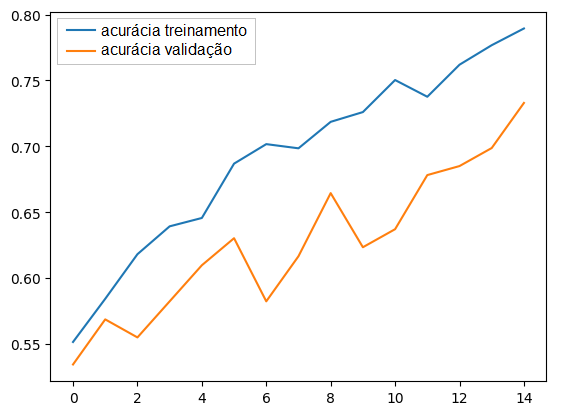
\includegraphics[width=\linewidth]{figuras/accuracy.png}
  \captionsetup{justification=centering}
  \vspace{-0.2cm}
  \\\textbf{\footnotesize Fonte: Elaborado pelos autores}
  \label{fig:acc10}
\end{minipage}\hfill
\begin{minipage}{0.45\textwidth}
  \centering
  \caption[\hspace{0.1cm}Grade Computacional.]{Gráfico de perda}
  \vspace{-0.4cm}
  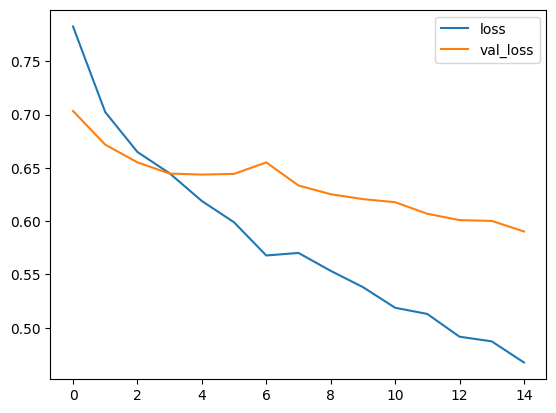
\includegraphics[width=\linewidth]{figuras/loss.png}
  \captionsetup{justification=centering}
  \vspace{-0.2cm}
  \\\textbf{\footnotesize Fonte: Elaborado pelos autores}
  \label{fig:loss10}
\end{minipage}
\end{figure}

Além disso, na Figura \ref{fig:loss10}, observa-se que o erro de treinamento diminui no decorrer das épocas, comportamento esperado, uma vez que quanto menor o erro, maior será a acurácia da predição. Em contrapartida, o erro de validação aumenta à medida que o número de épocas aumenta, levando assim à uma perda de generalização. Isso é um sinal de Sobreajuste (do inglês \textit{Overfitting}), comportamento indesejável de \textit{Machine Learning} que ocorre quando o modelo fornece previsões precisas para dados de treinamento, mas não para novos dados.


%%%%%%%%%%%%%%%%%%%%%%%     PREDIÇÕES       %%%%%%%%%%%%%%%%%%%%%%

\subsection{\esp Predição} \label{pred}

Por fim, foi feita a predição do modelo de classificação com dados de teste. 

O resultado da predição para um paciente sem câncer, disponível na Figura \ref{fig:predicao_sem}, retornou uma classificação correta, apontando que a imagem é de um paciente sem câncer. Entretanto, na Figura \ref{fig:predicao_com}, o modelo previu uma classificação incorreta, apontando que um paciente sem câncer tem a doença. Isso é devido à baixa acurácia que o modelo tem.

\begin{figure}[ht]
\centering
    \begin{minipage}[b]{0.45\textwidth}
        \centering
        \caption{Predição de paciente sem câncer}
        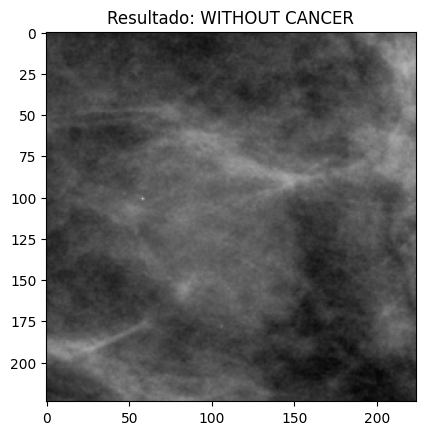
\includegraphics[width=\textwidth]{figuras/predicao_sem.png}
        \label{fig:predicao_sem}
         \textbf{\footnotesize Fonte: \href{https://www.kaggle.com/datasets/awsaf49/cbis-ddsm-breast-cancer-image-dataset}{\cite{newdatabase}}}
    \end{minipage}
    \hfill
    \begin{minipage}[b]{0.45\textwidth}
        \centering
        \caption{Predição de paciente com câncer}
        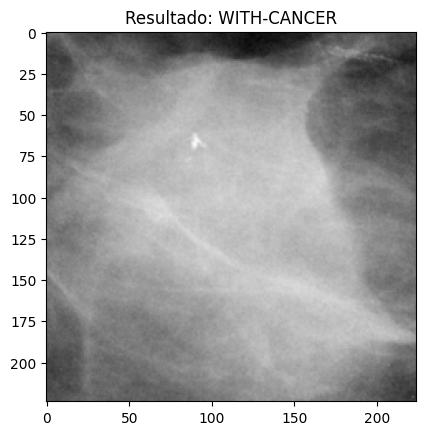
\includegraphics[width=\textwidth]{figuras/predicao_com.png}
        \label{fig:predicao_com}
        \textbf{\footnotesize Fonte: \href{https://www.kaggle.com/datasets/awsaf49/cbis-ddsm-breast-cancer-image-dataset}{\cite{newdatabase}}}
    \end{minipage}
\end{figure}
